% !Mode:: "TeX:UTF-8"

\chapter{VAE}

\section{隐变量模型}
我们使用如下的产生过程来生成样本$X$:从高维空间$\cal{Z}$中以概率$P(z)$采样一个向量$z$,该向量称为隐变量。基于隐变量$z$以概率$P(X|z;\theta)$采样得到样本$X$。则样本$X$产生的概率为:
\begin{displaymath}
P(X) = \int{P(X|z;\theta)}P(z)dz
\end{displaymath} 
在实际情况中样本$X$是容易获得的,而隐变量$z$则不是给定的。很多情况下我们需要给定样本$X$生成一个跟$X$类似的样本,这样我们就需要首先得到$X$对应的隐变量$z$,并基于此隐变量根据$P(X|z)$生成一个新的$X$。为了达到这样的目的,我们需要计算$P(z|X)$,根据贝叶斯公式我们有:
\begin{displaymath}
P(z|X) = \frac{P(z)P(X|z)}{\int{P(X|z;\theta)}P(z)dz} 
\end{displaymath} 
通过贝叶斯公式来直接得到隐变量的后验存在一个问题,我们需要对隐变量$z$进行积分,而这个积分在大多数情况下是不可计算的。
\section{VAE}
既然后验是难以直接计算的,那么基于变分的思想,我们可以引入一个新的分布$Q(z|X)$来对实际分布$P(z|X)$进行近似。我们希望新引入的$Q(z|X)$能够同$P(z|X)$分布尽可能的相似,故而可以最小化$Q(z)$和$P(z|X)$的KL距离来获得这个分布。
\begin{displaymath}
\begin{split}
KL(Q(z|X)\|P(z|X)) = E_{z \sim Q}(\log{Q(z|X)} - \log {P(z|X)})\\
KL(Q(z|X)\|P(z|X)) = E_{z \sim Q}(\log{Q(z|X)} - \log {P(X|z)-\log P(z)}) + \log P(X)\\
\log P(X) - KL(Q(z|X)\|P(z|X)) = E_{z \sim Q}(\log {P(X|z)}) -KL(Q(z|X) \| P(z)) 
\end{split}
\end{displaymath} 
该公式的左边包含两部分,一部分是$P(X)$也就是我们最终要最大化的那一项,另一部分是我们对$P(z|X)$的近似程度的一个损失,即对$z$的建模$Q(z|X)$同真实分布$P(z|X)$之间的差异。由于$KL(Q(z|X)\|P(z|X))$为正值,所以最大化第一项和第二项之和相当于最大化$P(z|X)$,同时最小化$KL(Q(z|X)\|P(z|X))$。右边同样包含两部分,第一部分是当$z$基于$Q(z|X)$建模时,基于$z$生成$X$的模型$P(X|z)$的信息量,第二部分则是相对于不包含任何关于样本$X$的分布$P(z)$,模型$Q(z|X)$中包含的关于$X$的信息量。对于公式的右边来说,第二部分可以看做一个将样本$X$通过模型$Q(z|X)$进行编码得到隐变量$z$,该隐变量$z$包含的关于$X$的信息量,而第一部分则是基于包含了$X$的信息的$z$,基于模型$P(X|z)$将$X$生成出来所需的额外的信息量。

由于$KL(Q(z|X)\|P(z|X))$为正值,故而$\log P(X) - KL(Q(z|X)\|P(z|X))$实际上是$\log P(X)$的一个ELOB下界:
\begin{displaymath}
\begin{split}
\log P(X) &= \log \int{P(X,z)}dz\\
&= \log \int{P(X,z)}\frac{Q(z|X)}{Q(z|X)} dz\\
&\geq \int{ Q(z|X) \log {\frac{P(X,z)}{Q(z|X)}} dz}\\
&= \int{ Q(z|X) \log {\frac{P(X|z)P(z)}{Q(z|X)}} dz}\\
&= \int{(\log P(X|z) - \log \frac{Q(z|X)}{P(z)})Q(z|X)dz}\\
&= E_{z \sim Q}(\log {P(X|z)}) -KL(Q(z|X) \| P(z))
\end{split}
\end{displaymath} 
由Jesen不等式成立条件得$Q(z|X) = P(z|X)$。

直接计算积分是不现实的,所以我们往往通过采样的方式来近似。不同于在分布$P(z)$上进行采样,新的ELOB下界的优化是通过在$Q(z|X)$上采样运算得到的。由于$P(z)$与$X$无关,所以采样得到的绝大多数$z$生成$X$的概率近乎为0,所以采样的效率非常低。而新的ELOB下界的优化则是在$Q(z|X)$上采样的,由于考虑了样本$X$的信息,从而可以使得采样得到的$z$能够更可能的产生$X$,提高了采样效率。

如图所示,假设$P(z)$为标准高斯分布${\cal{N}}(0,I)$,而$Q(z|X)$为均值为$\mu(X)$,方差为$\Sigma(X)$的高斯分布${\cal{N}}(\mu(X),\Sigma(X))$,则编码器$Q$基于给定的输入$X$生成均值$\mu(X)$和方差$\Sigma(X)$,而解码器$P$则从分布${\cal{N}}(\mu(X),\Sigma(X))$中采样一个$z$,并基于$z$产生一个$X'$。

\begin{figure}[htbp]
\centering
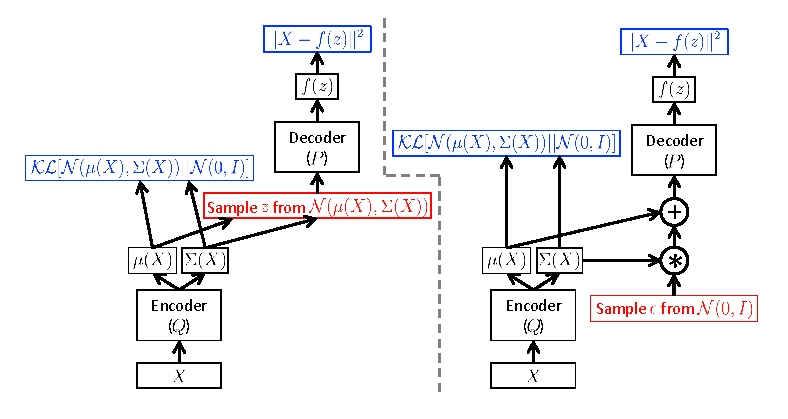
\includegraphics[width = 0.8\textwidth]{Vae_Reparameter}
\end{figure}
